
The method we employed to use \CP\ can be visualized in a four part
fashion, as depicted in \refFigure{fig:genView}. The first part, in
the upper level of the figure, shows the Selector, which selects a
set of values for the inlining parameters based on a strategy. The
second part, on the left, shows the Combined Profiling (\CP) process
applied to a program. The third part, at the bottom of the figure,
shows the execution test of a compiled program. And, in the center
of the figure we have the compiler.

\begin{figure}
  \centering
  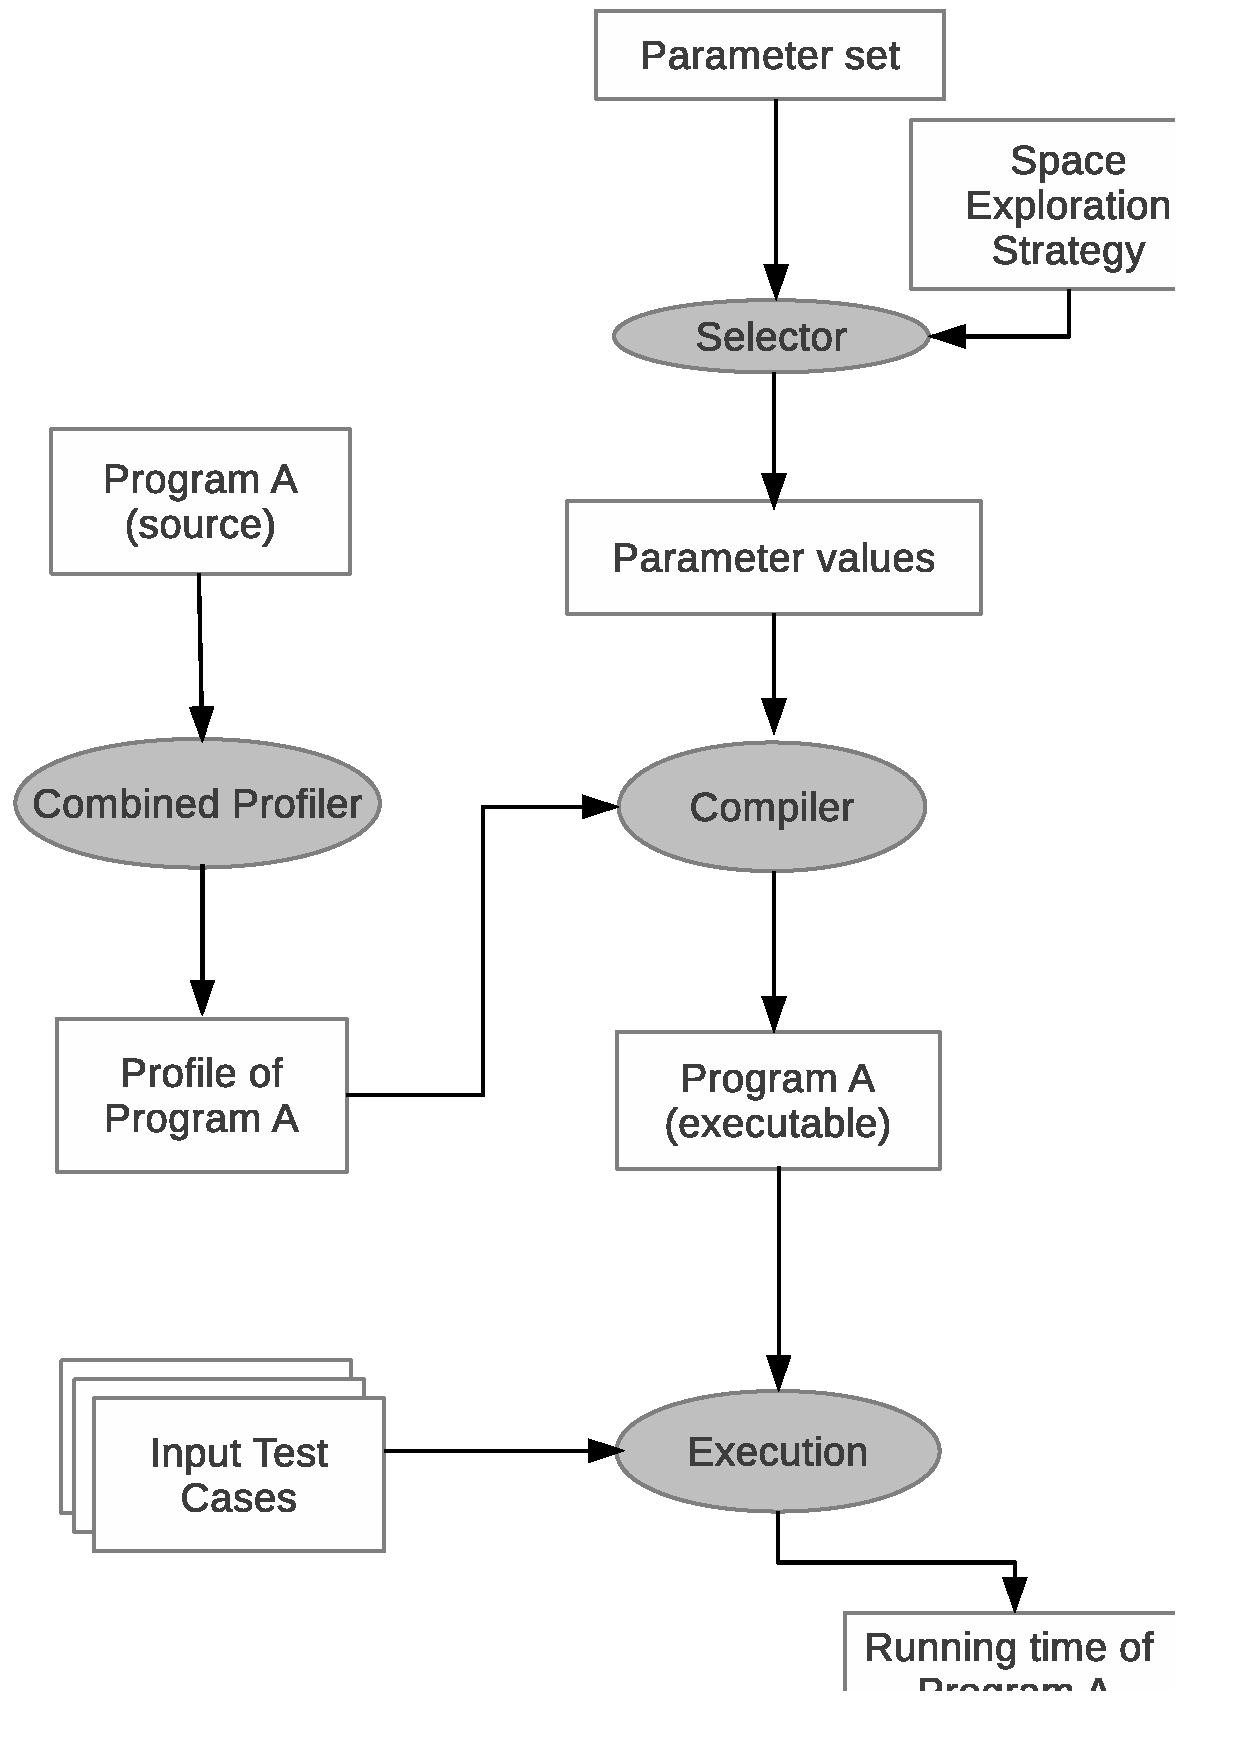
\includegraphics[width=0.50\linewidth]{Figures/genView}
  \caption{Generic view of the method}
  \label{fig:genView}
\end{figure}

We can use this method for parameter tuning, and also for a machine
learning approach trying to define the best set of parameters for
throughput or for latency. The process remains the same, we just have
to define properly what is a point of measure. More details on the
\CP\ profiling in \refFigure{fig:CPview}, whereas in \refFigure{CP:simple}
the simplified view is presented, the hatched area marks the \CP\
compiler; and in \refFigure{CP:expanded} the \CP\ compiler is shown in
more detail.

\begin{figure}
  \centering
  
  \begin{minipage}[t]{\linewidth}
    \subfigure[Simplified view of the process] {
      \begin{minipage}[b]{0.45\textwidth}
        \centering
        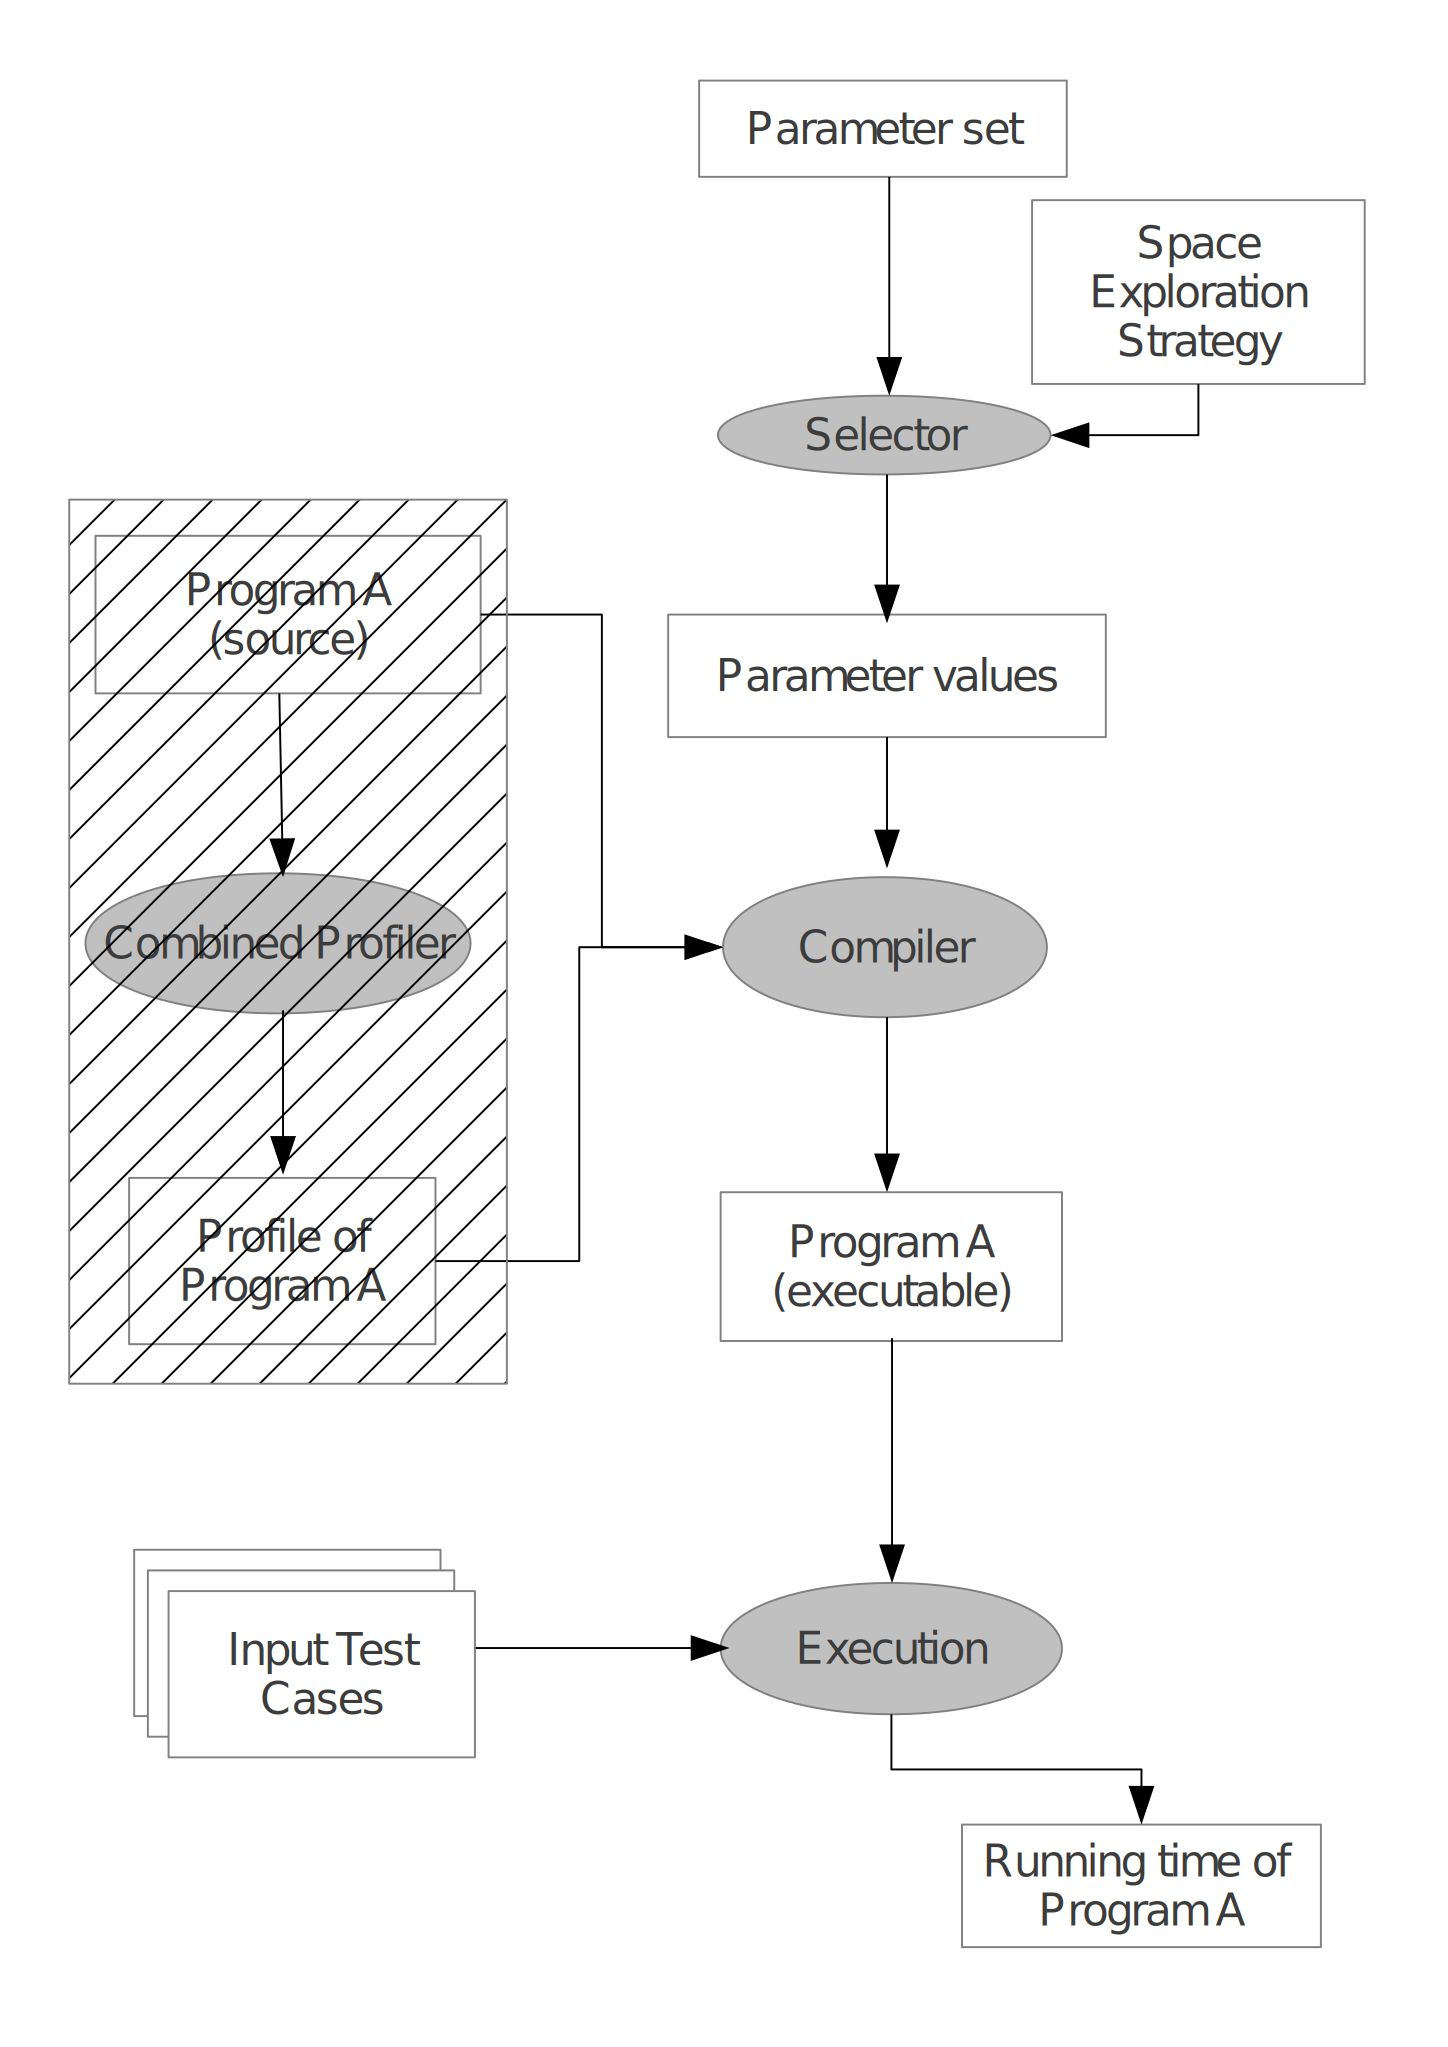
\includegraphics[height=12em]{Figures/CPview1}
      \end{minipage}
      \label{CP:simple}
    }
    \subfigure[Expanded view of the process] {
      \begin{minipage}[b]{0.45\textwidth}
        \centering
        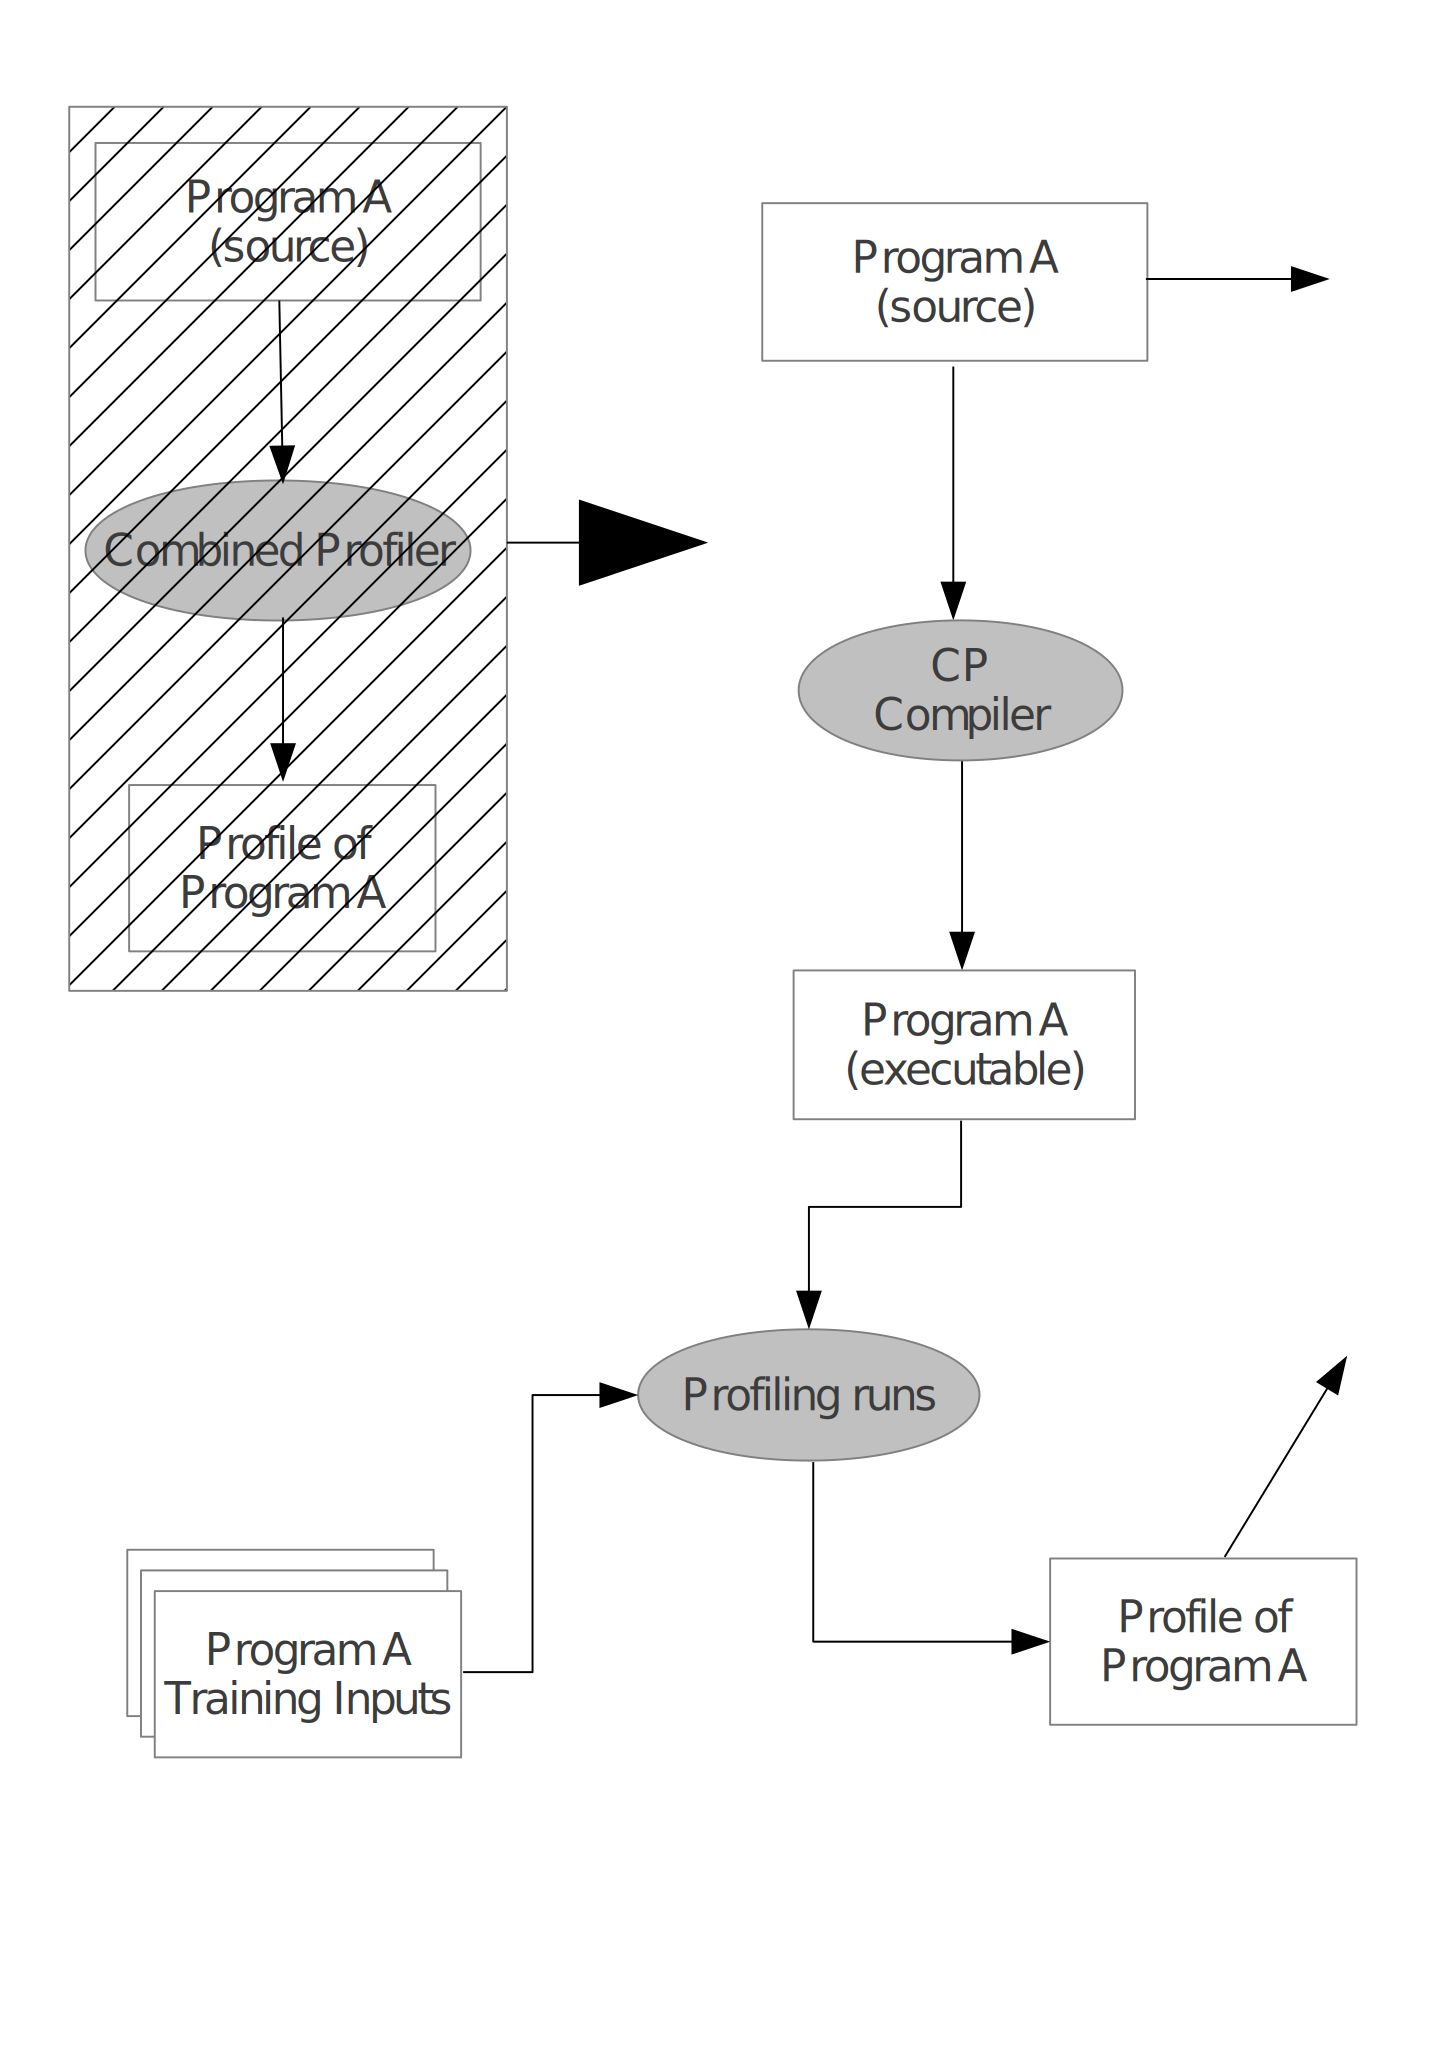
\includegraphics[height=12em]{Figures/CPview2}
      \end{minipage}
      \label{CP:expanded}
    }
  \end{minipage}
%    \vspace{1em}
%    \hrule
%    \vspace{1em}
  \caption{\CP\ compiler and the profile generation}
  \label{fig:CPview}
\end{figure}


In the case of parameter tuning, a point of measure is represented by
the set of parameter values of the compiler for the program under tuning
and its normalized value of the execution time for some test inputs. For
the machine learning case, a point of measure for throughput is the sum
of the execution times of each of the programs under test with its
associated parameter values. On the other hand for latency, a point of
measure is the geometric mean of the normalized values.

\subsection{Parameter Tuning}

Tuning compiler optimization options for a specific program is not an easy
task \cite{Zhong2009}. There exist some tools based on Genetic Algorithms,
Simulated Anealling \cite{Zhong2009}, Support Vector Machines \cite{SanchezCGO11},
etc. For the case of inlining a recently published research pointed to the
use of Neural Networks to induce effective inlining heuristics \cite{KulkarniCGO13}.
% Parameter tuning is a proficuous area of research.

As illustrated if \refFigure{fig:genView}, our method can be effetively used
to tune compiler optimization options; in this research we made an empirical
evaluation of it in the inlining case.

A set of parameter values that is suited to a benchmark, may achieve poor
results when applied to another benchmark. In Kulkarni \etal there
is a figure that illustrates this problem, in Figure 1 of \cite{KulkarniCGO13}
they show the sensitivity of callee size metric for various benchmarks.
Another difficult question to address is related to the interdependencies
found in the parameter set. Adjusting one parameter has some effects on
another, so it's not simple to tweak a set of parameter values.

Particularly considering the case of the callee size metric, it is commonly
used as threshold in many inlining algorithms, and, as mentioned above, the
best value for this parameter depends on the benchmark. This is the reason why
this parameter was not defined as a constant value in our approach, but as a
function that maps the callee size to a threshold value \cite{BerubePhD}.

As any inlining decision can have some impact on subsequent decisions, there
is a large space of possible inlining solutions, which can be traversed by
slightly changing values, thresholds in any metrics employed. In our case,
our space of possibilities can be traversed by changing the values of the
inlining parameters.

Referring again to Kulkarni \etal, we can actually visualise the problem
of searching the space for good solutions. As illustrated by Figure 2
in \cite{KulkarniCGO13}, the space is very large, but the set of good
solutions is limited to a small percentage of the whole space. It surely
is an indicator to the use of some AI algorithms to search for the optimal,
even sub-optimal solution. In our research, we need to find a sweet spot
where the parameter values fits best to a program making it run faster
than before for some benchmark inputs, that are representative for that
program.

Considering the effort usually employed by compiler writers in defining
and tuning a heuristic, our work presents a much more general approach
to the definition and tuning an inlining heuristic. First, it is
automatically parameterized in terms of some common thresholds like the
callee size, which is represented by function on the actual callee size,
whose output is used to limit the code-growth budget. Second, it allows
an automatic procedure for tuning in the parameters of the inliner.

The Hypothesis we use is that most inlining candidates that significantly
impact the performance of any run also improve performance across
most of the workload.  The number of inlining opportunities that are
particularly important for only a minority of runs is a small
fraction of the total number of inlining opportunities that
significantly impact program performance \cite{BerubePhD}.
